\subsection{Đánh giá hiệu năng}

Trong quá trình phát triển trò chơi multiplayer 3D \textit{Fishy Business}, nhóm nhận thấy rằng hiệu năng hệ thống đóng vai trò rất quan trọng đối với trải nghiệm người chơi. Do trò chơi hoạt động trong môi trường multiplayer thời gian thực, đồng thời phải xử lý nhiều hệ thống như rendering môi trường 3D, animation, UI, networking, voice chat và particle effect, hiệu năng có thể bị ảnh hưởng đáng kể nếu không được tối ưu hợp lý.

Để đánh giá hiệu năng của trò chơi, nhóm sử dụng Unity Profiler và Statistics Window để theo dõi các thông số như số lượng Draw Calls, tốc độ khung hình FPS (Frames Per Second), mức sử dụng CPU/GPU và độ ổn định của hệ thống trong quá trình gameplay. Việc kiểm tra được thực hiện trên nhiều phiên chơi multiplayer thực tế nhằm mô phỏng điều kiện hoạt động của trò chơi khi có nhiều người chơi cùng tham gia.

Sau đây, nhóm sẽ tiến hành đánh giá hiệu năng hệ thống dựa trên một phiên chơi thực tế với 3 người chơi, được thực hiện trên thiết bị và mạng có cấu hình như sau:
\begin{itemize}
    \item Cấu hình thiết bị:
        \begin{itemize}
            \item Hệ điều hành: Windows 11 Home Single Language 64-bits
            \item Bộ xử lý: Intel Core 7 150U (10 nhân, 12 luồng, xung nhịp 1.80 GHz)
            \item Bộ nhớ RAM: 16 GB
            \item Card đồ họa: Intel Graphics hỗ trợ DirectX 12
            \item Kiến trúc hệ thống: x64-based PC
            \item Thiết bị: Dell Inspiron 14 5440
        \end{itemize}
    \item Cấu hình mạng:
        \begin{figure}[H]
            \centering
            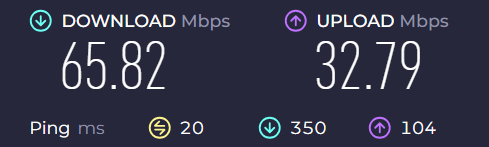
\includegraphics[width=0.7\linewidth]{11.Thu thập dữ liệu người dùng và đánh giá/hieu-nang/network.png}
            \caption{Cấu hình mạng}
        \end{figure}
\end{itemize}


\subsubsection{Hiệu năng trước khi tối ưu}

Ở giai đoạn đầu phát triển, nhóm chủ yếu tập trung vào việc hoàn thiện gameplay và các tính năng multiplayer cốt lõi nên chưa tiến hành tối ưu rendering hoặc batching object. Trong điều kiện này, hiệu năng tại màn hình chính tương đối ổn định do số lượng object trong scene còn ít và chưa có nhiều tương tác phức tạp.

Kết quả đo đạc cho thấy tại màn hình chính:
\begin{itemize}
    \item Draw Calls duy trì ở mức khoảng 30.
    \item FPS dao động trong khoảng 70--80 FPS.
\end{itemize}

Tuy nhiên, khi người chơi chuyển sang gameplay multiplayer, hiệu năng bắt đầu giảm đáng kể. Nguyên nhân là do scene gameplay chứa nhiều object cần render đồng thời, bao gồm nhân vật người chơi, môi trường 3D, UI gameplay, animation và các hiệu ứng particle. Ngoài ra, hệ thống multiplayer liên tục thực hiện việc synchronize dữ liệu giữa các client, làm tăng thêm tải xử lý cho CPU.

Qua quá trình phân tích bằng Unity Profiler, nhóm nhận thấy số lượng Draw Calls tăng rất mạnh trong gameplay. Ở trạng thái chơi thông thường, số lượng Draw Calls dao động khoảng 800. Trong một số trường hợp có nhiều người chơi xuất hiện cùng lúc hoặc có nhiều hiệu ứng được kích hoạt đồng thời, số lượng Draw Calls có thời điểm tăng lên hơn 1300.

Khi số lượng Draw Calls tăng quá cao, CPU phải liên tục gửi lệnh render tới GPU, dẫn đến hiện tượng nghẽn cổ chai trong pipeline rendering. Điều này làm FPS giảm xuống chỉ còn khoảng 40--50 FPS. Trong quá trình chơi thực tế, trò chơi bắt đầu xuất hiện hiện tượng khựng hình nhẹ, giảm độ mượt khi di chuyển camera hoặc khi nhiều người chơi tương tác đồng thời trong cùng một khu vực.

Nguyên nhân chính của vấn đề này đến từ:
\begin{itemize}
    \item Các object sử dụng nhiều material khác nhau nên không thể batching.
    \item Mỗi mesh được render riêng lẻ dẫn đến số lượng Draw Calls tăng cao.
    \item Hệ thống UI gameplay liên tục rebuild Canvas.
    \item Một số object và effect được Instantiate/Destroy thường xuyên gây Garbage Collection.
\end{itemize}

\begin{figure}[H]
    \centering
    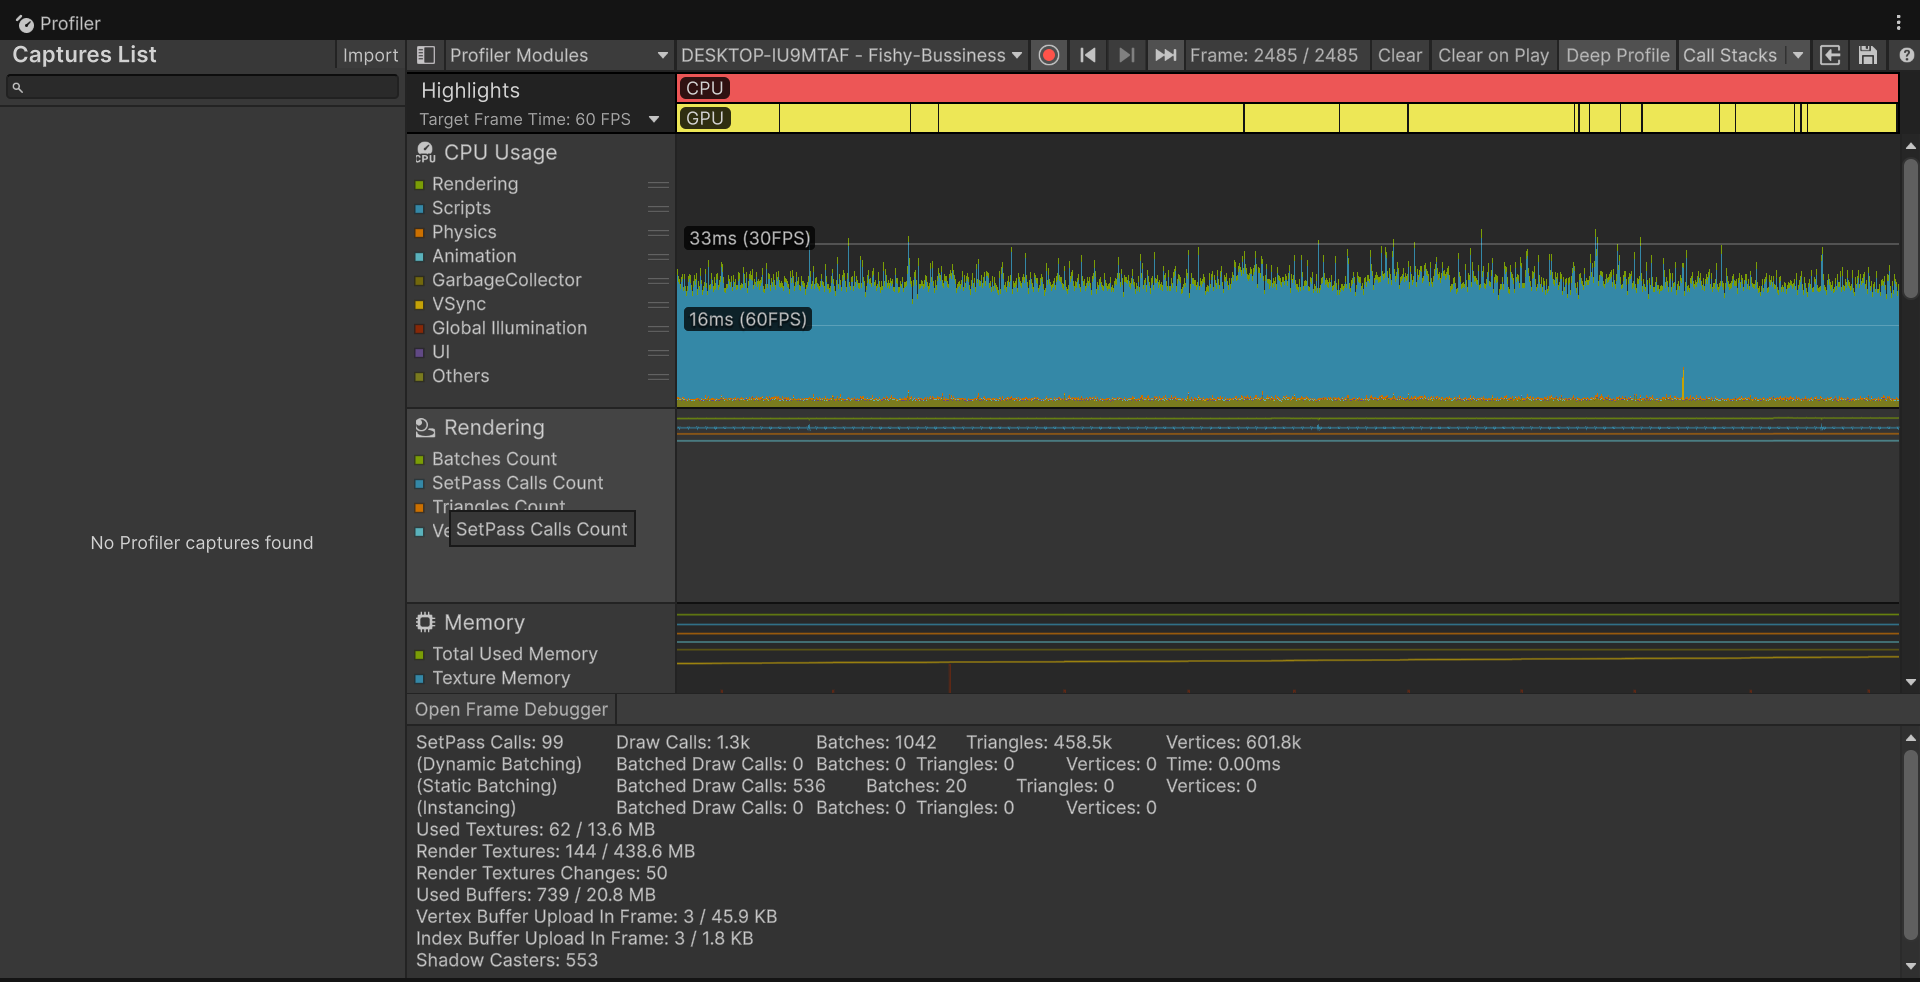
\includegraphics[width=0.8\linewidth]{11.Thu thập dữ liệu người dùng và đánh giá/hieu-nang/drawCallGameplay_Old.png}
    \caption{Hiệu năng gameplay trước khi tối ưu}
    \label{fig:performance_before}
\end{figure}

Từ kết quả trên, nhóm nhận thấy rằng nếu không thực hiện tối ưu hóa, trò chơi sẽ khó có thể đảm bảo trải nghiệm ổn định trong các phiên multiplayer nhiều người chơi.

\subsubsection{Quá trình tối ưu hiệu năng}

Sau khi xác định được nguyên nhân gây giảm hiệu năng, nhóm tiến hành áp dụng nhiều kỹ thuật tối ưu khác nhau nhằm giảm tải cho CPU và GPU trong quá trình rendering.

Đầu tiên, nhóm tiến hành tối ưu hệ thống rendering bằng cách áp dụng \textit{Static Batching} đối với các object tĩnh trong môi trường như bàn chơi, tường, vật trang trí và nội thất. Việc này giúp Unity có thể gộp nhiều mesh thành một Draw Call duy nhất thay vì render riêng lẻ từng object.

Bên cạnh đó, đối với các object xuất hiện lặp lại nhiều lần như thẻ bài, vật phẩm hoặc các props trang trí, nhóm sử dụng \textit{GPU Instancing} để GPU có thể render nhiều object giống nhau trong cùng một lần gọi. Kỹ thuật này giúp giảm đáng kể số lượng Draw Calls trong gameplay.

Ngoài ra, nhóm cũng tiến hành gộp texture và sử dụng chung material giữa các object tương tự. Trước khi tối ưu, nhiều object sử dụng material riêng biệt khiến Unity không thể thực hiện batching hiệu quả. Sau khi áp dụng Texture Atlas và Material Sharing, số lượng Draw Calls giảm đáng kể.

Hệ thống UI cũng được tối ưu bằng cách chia nhỏ Canvas thay vì sử dụng một Canvas lớn cho toàn bộ giao diện gameplay. Điều này giúp giảm số lần rebuild UI mỗi khi có thay đổi nhỏ trong giao diện.

Ngoài phần rendering, nhóm cũng tối ưu networking bằng cách:
\begin{itemize}
    \item Chỉ synchronize những dữ liệu gameplay thực sự cần thiết.
    \item Giảm tần suất cập nhật của các object không quan trọng.
    \item Hạn chế gửi RPC không cần thiết giữa các client.
\end{itemize}

Việc giảm lượng network update giúp CPU có thêm tài nguyên cho rendering và gameplay logic.

\subsubsection{Hiệu năng sau khi tối ưu}

Sau khi áp dụng các kỹ thuật tối ưu, hiệu năng của trò chơi được cải thiện rõ rệt. 
Ở màn hình chính, FPS tăng từ 70 lên đến 100, còn số lượng Draw Calls có giảm nhưng không đáng kể.
Còn khi đang trong phòng chơi thì số lượng Draw Calls giảm xuống còn khoảng 200--300, thấp hơn rất nhiều so với mức 800--1300 trước đó.

Nhờ việc giảm số lượng Draw Calls và batching các object hiệu quả hơn, FPS của trò chơi cũng được cải thiện đáng kể. Trong các phiên chơi multiplayer thực tế, FPS duy trì ổn định trong khoảng 60--70 FPS ngay cả khi có nhiều người chơi cùng hoạt động trong scene.

Ngoài việc FPS tăng lên, nhóm cũng nhận thấy:
\begin{itemize}
    \item Hiện tượng tụt FPS đột ngột giảm đáng kể.
    \item Gameplay trở nên mượt hơn trong quá trình di chuyển và tương tác.
    \item Frame time ổn định hơn so với trước khi tối ưu.
    \item CPU usage giảm đáng kể trong quá trình rendering.
\end{itemize}

Việc batching object và giảm số lượng material được xem là nguyên nhân chính giúp cải thiện hiệu năng của hệ thống. Khi số lượng Draw Calls giảm, CPU không còn phải xử lý quá nhiều lệnh render trong mỗi frame, từ đó giúp tốc độ xử lý khung hình ổn định hơn.

\begin{figure}[H]
    \centering
    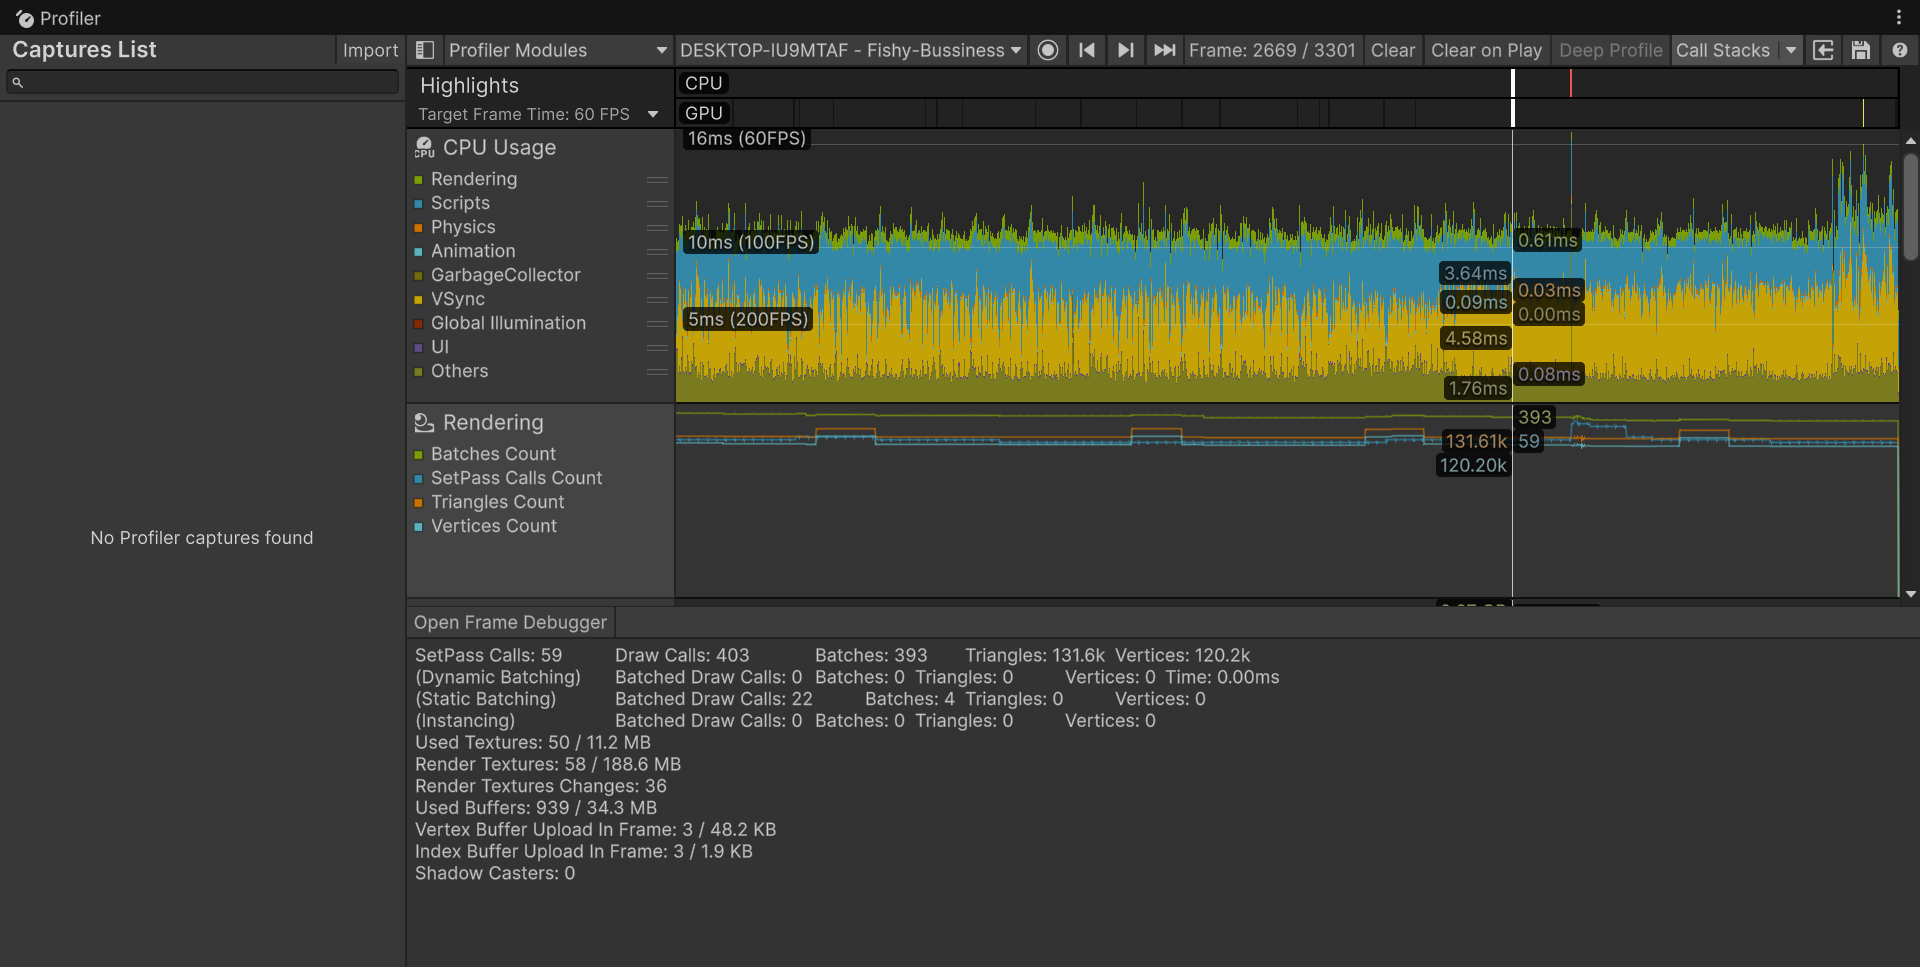
\includegraphics[width=0.8\linewidth]{11.Thu thập dữ liệu người dùng và đánh giá/hieu-nang/drawCallGameplay_New.png}
    \caption{Hiệu năng gameplay sau khi tối ưu}
    \label{fig:performance_after}
\end{figure}

\subsubsection{Đánh giá kết quả}

Kết quả thử nghiệm cho thấy các kỹ thuật tối ưu hóa đã mang lại hiệu quả rõ rệt đối với hệ thống multiplayer của trò chơi. So với phiên bản ban đầu, số lượng Draw Calls đã giảm khoảng 70\%, đồng thời FPS được duy trì ổn định hơn trong quá trình chơi.

Qua quá trình tối ưu hiệu năng, nhóm hiểu rõ hơn về cách Unity xử lý rendering pipeline, ảnh hưởng của Draw Calls đối với CPU và vai trò của batching trong việc tối ưu hiệu năng trò chơi. Ngoài ra, nhóm cũng tích lũy được nhiều kinh nghiệm thực tế trong việc tối ưu hóa game multiplayer 3D, đặc biệt là trong các tình huống có nhiều object và người chơi hoạt động đồng thời trong cùng một scene.

Những kết quả đạt được cho thấy việc tối ưu rendering và quản lý tài nguyên là một bước rất quan trọng trong quá trình phát triển các trò chơi multiplayer thời gian thực, góp phần đảm bảo tính ổn định và cải thiện trải nghiệm người chơi trên nhiều cấu hình phần cứng khác nhau.